\documentclass[10pt,a4paper]{article}
\usepackage[latin1]{inputenc}
\usepackage{amsmath}
\usepackage{amsfonts}
\usepackage{amssymb}
\usepackage{graphicx}
\usepackage{multicol}
\usepackage{changepage}
\usepackage{float}
\usepackage{cite}
\usepackage{url}
\usepackage{imakeidx}
\makeindex

\usepackage[left=2.50cm, right=2.50cm]{geometry}
\usepackage[spanish]{babel}

\author{Axel}
\title{Portada siempre practica}

\begin{document}
%encabezado 
\pagestyle{plain}{
\pagestyle{empty}
\changepage{3cm}{1cm}{-0.5cm}{-0.5cm}{}{-2cm}{}{}{}
\noindent

%sEGIUN EL formato de sus imagenes, deben encontrar una configuracion adeacuada para ustedes
{\small
\begin{tabular}{p{0.626\textwidth} p{0.50\textwidth} }

\includegraphics[scale=0.26]{uaem.jpg} &  
\includegraphics[scale=0.3]{ico.jpg}
\end{tabular}
}

%datos de la caratula
\begin{center}
\par\vspace{2cm} %Rspacoo dejado antes del encabezado
{
\Huge\textbf{
Universidad Aut\'onoma del Estado de Mex\'ico \\[1cm] Ingenieria en Computaci\'on
}
}
\par\vspace{1.5cm}
{
\Large\textbf{ Materia: Redes Neuronales \\ Compuertas	l\'ogicas	con	perceptr\'on	simple
}
}
\par\vspace{1.5cm}
{
\large\textbf{Axel Valenzuela Ju\'arez \\Profesor: Dr. Asdr\'ubal	L\'opez	Chau \\ 31 de Octubre del 2019  } 
}

\par\vspace{1.5cm}

\end{center}
\clearpage

}

\printindex

\section{
Introducci\'on a redes multicapa
}
\subsection{Compuertas Logicas}
Los circuitos integrados digitales est\'an formados por resistencias, diodos y
transistores, montados en silic\'on u otro semiconductor conocido como sustrato.
Cada uno de los integrados contiene varias compuertas l\'ogicas.
Las tres operaciones l\'ogicas b\'asicas son And Or y Not.
Los s\'imbolos que se utilizan para representar a cada una se pueden observar en la Fig:\ref{fig:Compuertas}


\begin{figure}[H]
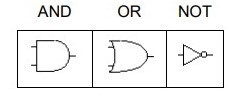
\includegraphics[scale=1] {compuertas.jpg}
\caption{Compuertas And, Or ,Not.}
\label{fig:Compuertas}
\end{figure}

\paragraph{Cada compuerta tiene su tabla de verdad , la cual indica cuando habra voltaje y cuando no, siendo 1 voltaje y 0 sin voltaje, ver Fig:\ref{fig:tablas}}

\begin{figure}[H]
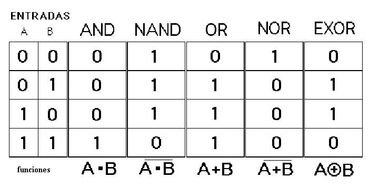
\includegraphics[scale=0.7] {tablas.jpg}
\caption{Tablas de verdad.}
\label{fig:tablas}
\end{figure}

\subsection{El perceptron}

\paragraph{Para aplicar el perceptr\'on es necesario determinar los vectores de W, un perceptr\'on recibe dos entradas y un vector w para as\'i obtener una salida, se puede ver la representaci\'on de un perceptr\'on a continuaci\'on. Fig: \ref{fig:Rperceptron} }
\begin{figure}[h]
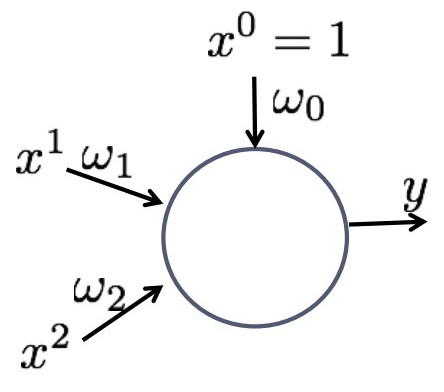
\includegraphics[scale=0.4] {RepPerc.jpg}
\caption{Representaci\'on de un perceptr\'on.}
\label{fig:Rperceptron}
\end{figure}

\paragraph{El algoritmo que ocupa el perceptr\'on es muy simple ya que se compone de dos for y un if y su respectivo else, se multiplica el vector W por el vector X, para poder multiplicarlos se necesita sacar la transpuesta de W, y despu\'es simplemente se compara el resultado, si el resultado es mayor que 0 se le asigna el valor de 1 a $"y"$ y si es menor se le asigna un 0.}

\section{Desarrollo}
\paragraph{Se uso el mismo algoritmo del perceptr\'on, solo se crearon un conjunto de datos por medio de np.ramdom.uniform, para ello se dio un rango de n\'umeros a generar  de 0 a 0.3 y de 0.7 a 1,
los datos quedan ordenados de la manera que quedaban en el anterior ejercicio. Fig: \ref{fig:and}}

\begin{figure}[h]
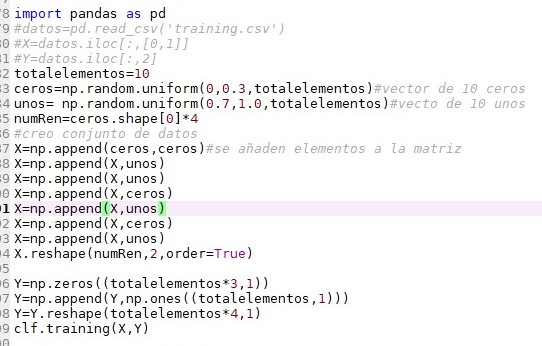
\includegraphics[scale=0.7] {and.jpg}
\caption{Creacion de datos de prueba.}
\label{fig:and}
\end{figure}

\paragraph{El algoritmo entrenara al perceptr\'on para que de como resultados sus tablas de verdad}

\paragraph{Este mismo procedimiento se tiene que realizar para cada compuerta excepto en el caso de la compuerta not ya que en esa compuerta una entrada siempre ser\'a 0 para que simplemente se niegue.}

\section{Conclusion}
\paragraph{En conclusi\'on fue un gran avance lograr utilizar múltiples neuronas para solucionar un problema como el de la xor, abriendo paso a un gran avance tecnol\'ogico, es necesario aprender a unir m\'ultiples neuronas para comprender el funcionamiento de estas, hoy en d\'ia existen m\'ultiples programas que pueden hacer esto de manera muy r\'apida pero siempre es importante comprender el funcionamiento de lo que hay detr\'as , para lograr innovar, al fin del d\'ia eso es lo que hace al ingeniero.}
\paragraph{Tengo que destacar que este tema se me complico m\'as de lo que pensaba por la falta de tiempo, y talvez comprensi\'on a la hora de utilizar las compuertas , la manera en c\'omo funcionan las entradas de ellas y los datos a utilizar para el testing y entrenamiento.}

\section{Referencias}
\paragraph{Fern\'andez, J. L. (2003). L\'ogica Computacional. En \'A. M. Riesco. UNED.}
\paragraph{VEGA, J. L. (2012). L\'ogica Computacional. Estado de M\'exico: Red Tercer Milenio.}

\end{document}